\documentclass[tikz,border=10pt]{standalone}
\usepackage{tikz}
\usetikzlibrary{angles,quotes,calc}
\usepackage{tkz-euclide} %for right angle marker

\begin{document}
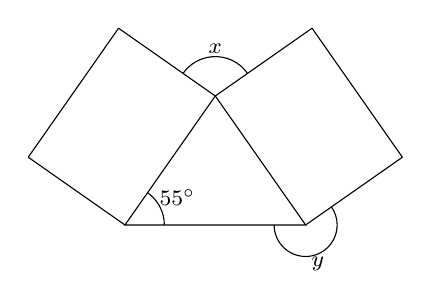
\begin{tikzpicture}[scale = 1]
    % Initial point
    \coordinate (A) at (0,0);
    % Draw isoceles triangle
    \draw (A) -- ++(55:2cm) coordinate (B) -- ++(-55:2cm) coordinate (C) -- cycle;

    % Draw square 1
    \draw (A) -- ++(145:1.5cm) coordinate (K);
    \draw (B) -- ++(145:1.5cm) coordinate (L);
    \draw (K) -- (L);
    %square 2
    \draw (C) -- ++(35:1.5cm) coordinate (M);
    \draw (B) -- ++(35:1.5cm) coordinate (N);
    \draw (M) -- (N);
    
    % Draw the angle between lines
    \pic [draw, "\footnotesize $55^\circ$ ", angle eccentricity=1.5, angle radius=0.5cm] {angle = C--A--B};
    \pic [draw, "\footnotesize $x$", angle eccentricity=1.2, angle radius=0.5cm] {angle = N--B--L};
    \pic [draw, "\footnotesize $y$", angle eccentricity=1.3, angle radius=0.4cm] {angle = A--C--M};
   

\end{tikzpicture}
\end{document}

